% Requires \usepackage{graphicx}. Paths are relative to the project root.

\begin{figure}[htbp]
\centering
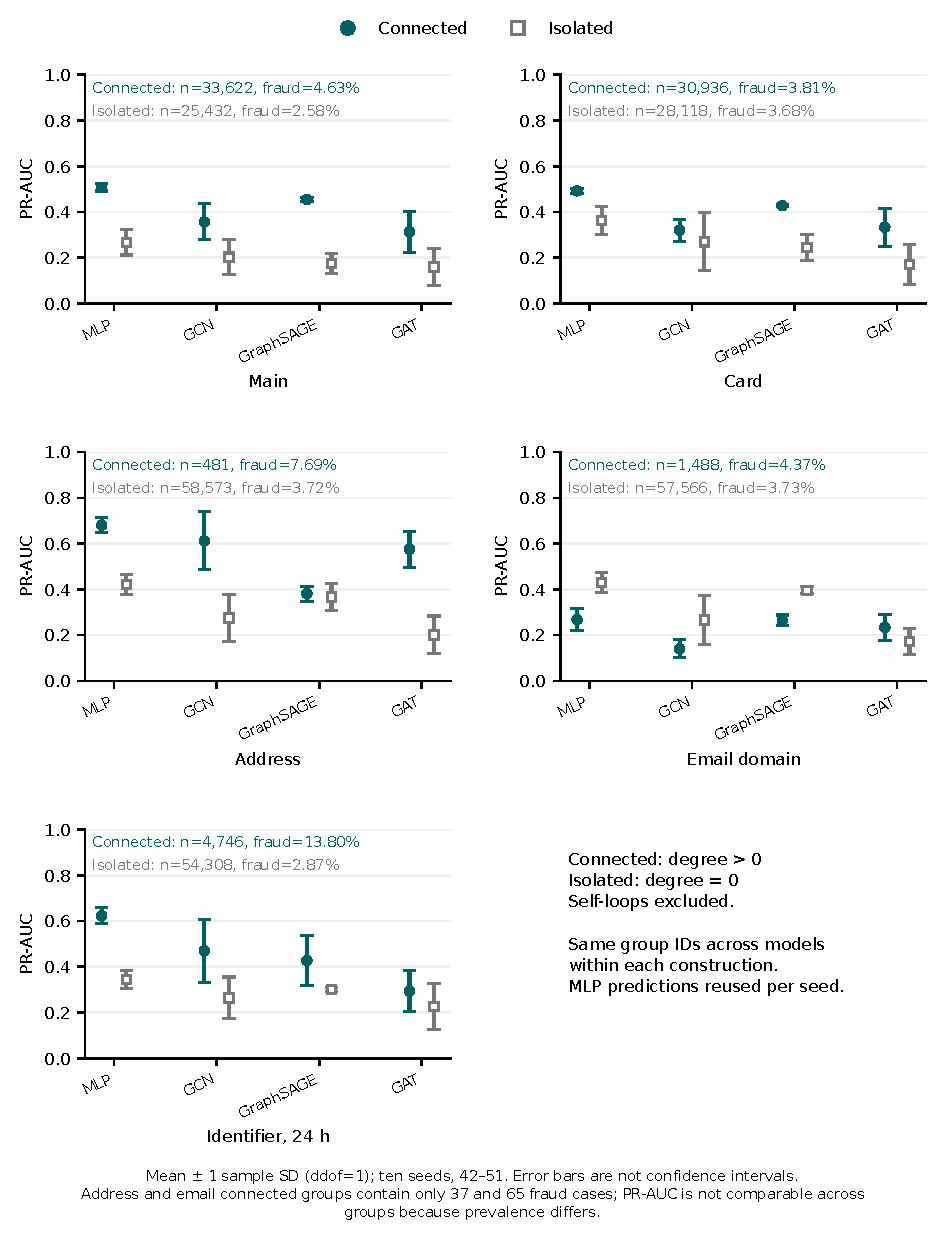
\includegraphics[width=\linewidth]{thesis_figures/06_connected_vs_isolated.pdf}
\caption{IEEE-CIS connected/isolated AP on identical test IDs across models within each construction. Ten-seed means $\pm$ sample SD; group sizes and fraud rates are shown. Degree excludes self-loops. Address and email connected groups contain only 37 and 65 fraud cases; PR-AUC is not comparable across groups because prevalence differs. MLP predictions are reused across constructions.}
\label{fig:06-connected-vs-isolated}
\end{figure}

\begin{figure}[htbp]
\centering
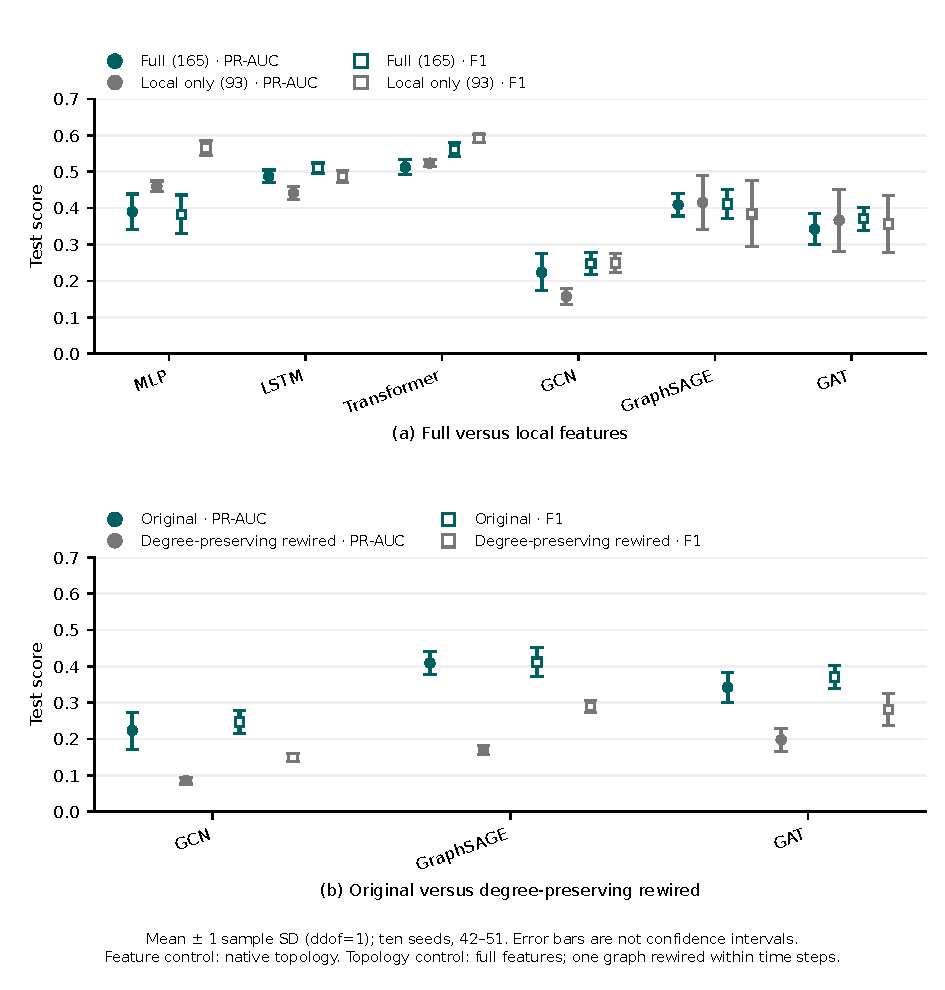
\includegraphics[width=\linewidth]{thesis_figures/07_elliptic_feature_topology_controls.pdf}
\caption{Elliptic controls: full (165) versus local-only (93) features for all six models; original versus degree-preserving rewired topology for the three GNNs. Circles show AP, open squares F1. Mean $\pm$ sample SD over seeds 42--51. Rewired edges remain within time steps; full feature values are retained. One graph seed, 20261013, is reused, so error bars measure training-seed variation, not graph-realization variation. Original historical runs and the validated sparse GNN control backend can differ in floating-point reduction order.}
\label{fig:07-elliptic-feature-topology-controls}
\end{figure}
